Consider the image and it's objects in Figure \ref{fig:introPhoto}. Even though the person on the right is comparable in size to the left person, he is remembered far less by humans (indicated by their memorability scores of $0.18$ and $0.64$ respectively). Many humans tend to remember the fish in the center and the person on the left even after a $30$ minute duration (memorability score $= 0.64$). Interestingly, despite covering a large portion of the image, the boat is also remembered far less by humans (memorability $= 0.18$). 

While recent studies related to image memorability have shed light on the large differences that exist between the memorabilities of different images, and the intrinsic and extrinsic properties that make an image memorable, the above example raises an interesting question: what exactly about an image is remembered?  Need to highlight why this will be important to study for a computer vision standpoint and memorability literature viewpoint. Maybe point that image memorability is an interesting problem, can be predicted by comp vis algos, has applicability such as modfying of photographs based on memorability. The example in Figure \ref{fig:introPhoto} suggests that there exists significant and interesting differences in memorability of objects in an image previously not studied in the literature. knowing about object memorability can lead to a clear understanding of the specific components of an image that drive memorability is still unknown.







In this paper, we systematically explore the memorability of objects within individual images and shed light on the various factors and properties that drive object memorability.


Despite progress in the computer vision literature on image memorability, a clear understanding of the specific components of an image that drive memorability is still unknown.


Firstly, our work explores if object memorability is a property shared across subjects and answers - can specific objects inside an image can be memorable to all of us? Next, I want to quantify which objects in general are most memorable and which ones are least memorable. This could lead to interesting questions like if an image contains highly memorable objects, could it's memorability still be low? Another way would be think can an image still be memorable even if the objects inside it have low memorability? Not only am I curious about this question, I believe that this will be very beneficial for object detection algorithms. For example, classes like person, dogs are easy to detect for current state-of-the-art computer vision algorithms but objects like chairs, bottles are very hard to detect. Could there be a correlation between the two? Are classes like chair and bottles tough to detect because these objects are less memorable? If there is, then object detection algorithms could use memorability as one of the features to improve the detection performance in future. Lastly, I want to study the correlation between salient objects and memorable objects. Are objects that are more salient, easier to memorize as well? Finding the overlap and differences between saliency and memorability would go a long way to help object detection algorithms.

Can specific objects inside an image be memorable to all of us and can we better understand the properties that drive object memorability within individual images?



 
 no study has systematically explored memorability of objects within individual images. Inspired by this, here, we are not just interested in understanding image memorability, we are interested in understanding memorability of objects in an image. Can some objects in individual images be more memorable to us and can we estimate their predictability?  And how exactly do different objects matter, whether it be size, spatial arrangement, etc.

%Studies related to long-term memory have demonstrated that humans have a remarkable ability to remember a large amount of visual information and thousands of different pictures even after seeing each of them only once.  Recent studies related to image memorability have shown that
%
%
%Human long-term memory can store a remarkable amount of visual information and remember thousands of different pictures even after seeing each of them only once [25, 1]. However, it appears to be the fate of visual memories that they degrade [13, 30]. While most of the work in visual cognition has examined how people forget for general classes of visual or verbal stimuli [30], little work has looked at which image information is forgotten and which is retained. Does all visual information fade alike? Are there some features, image regions or objects that are forgotten more easily than others? Inspired by work in visual cognition showing that humans selectively forget some objects and regions from an image while retaining others [22], we propose a novel probabilistic framework for modeling image memorability, based on the fading of local image information.

\begin{figure}[t]
\centering
\subfigure{\centering 
\includegraphics[width=0.4\textwidth]{figures/introduction/113.jpg}} 

\vspace{-3mm}

\subfigure{\centering 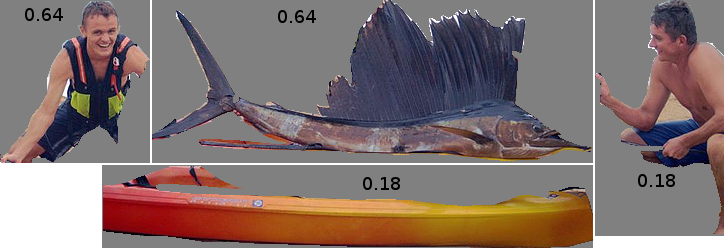
\includegraphics[width=0.4\textwidth]{figures/introduction/allObs.png}}
\vspace{-5mm}\caption{\footnotesize\textbf{Memorability of different objects.} Memorability scores of objects for the image in the top row obtained from our pysophysics experiment. }\label{fig:introPhoto}
\end{figure}

%Recent work on image memorability [6, 7, 12] has shown that there are large differences between the memorabilities of different images, and these differences are consistent across context and observers, suggesting that memory differences are intrinsic to the images themselves. Using machine learning tools such as support vector regression and a fully annotated dataset of images with human memorability scores, Isola et al [7] show that an automatic image ranking algorithm matches individual image memory scores quite well: with dynamic scenes with people interacting as most memorable, static indoor environments and human-scale objects as somewhat less memorable, and outdoor vistas as forgettable. In addition, using manual annotation, Isola et al. quantified the contribution of segmented regions to the image memorability score, creating a memorability map for each individual image that identifies objects that are correlated with high or low memorability scores. However, this previous work did not attempt to discover in an automatic fashion which part of the
%image is memorable and which regions are forgettable.
%
%In this paper, we introduce a novel framework for predicting image memorability that is able to
%account for how memorability of image regions and different types of features fade over time, offering memorability maps that are more interpretable than [7]. The current work offers three original contributions: (1) a probabilistic model that simulates the forgetting local image regions, (2) the automatic discovery of memorability maps of individual images that reveal which regions are memorable/ forgettable, and (3) an improved overall image memorability prediction from [7], using an automatic, data-driven approach combining local and global images features. 

%http://cvcl.mit.edu/papers/IsolaXiaoTorralbaOliva-PredictingImageMemory-CVPR2011.pdf​ ​ In summary, in this paper, a large dataset of images is released wherein the authors ran experiments on human subjects and quantified how memorable each image is. They also ran various analysis on what makes an image more memorable than others. For example, aesthetically pleasing images like landscapes etc are less memorable than an image containing a person. Subsequently, they have showed using computer vision algorithms that they can predict the memorability of images automatically with high accuracy.
%
%http://web.mit.edu/jxiao/Public/publication/2012/NIPSmemorability/paper.pdf​ is a follow up work done by the same authors and is related to memorability of regions in an image i.e. some regions in an image will be more memorable than others. If you go to Figure 4 (pg 7), the authors have built 'memorability maps' for each image via computer vision algorithms. Basically this means that for every pixel (and consequently a region) in an image, their algorithm outputs a memorability value. They then used these memorability maps to predict image memorability from the dataset in the first paper with even greater accuracy. Do note that they have not collected any actual ground truth memorability maps i.e. we still don't know what regions/objects humans consider more memorable in an image.
%
%Following up from this paper, I am interested in not just understanding image memorability, I am interested in understanding memorability of objects in an image. Firstly, I want to see if object memorability is shared across subjects and study if objects remembered by one person are also likely to be remembered by others and vice versa. Next, I want to quantify which objects in general are most memorable and which ones are least memorable. This could lead to interesting questions like if an image contains highly memorable objects, could it's memorability still be low? Another way would be think can an image still be memorable even if the objects inside it have low memorability? Not only am I curious about this question, I believe that this will be very beneficial for object detection algorithms. For example, classes like person, dogs are easy to detect for current state-of-the-art computer vision algorithms but objects like chairs, bottles are very hard to detect. Could there be a correlation between the two? Are classes like chair and bottles tough to detect because these objects are less memorable? If there is, then object detection algorithms could use memorability as one of the features to improve the detection performance in future. Lastly, I want to study the correlation between salient objects and memorable objects. Are objects that are more salient, easier to memorize as well? Finding the overlap and differences between saliency and memorability would go a long way to help object detection algorithms.
%
%The challenge however would be obtaining ground truth memorability of objects. The ideal scenario would be to get how memorable each object is for each image for all the subjects in a database. If we were to successfully collect and build a database which tells us which regions/objects are more memorable in an image, we could be able to answer all of the above questions. Let's try to talk in more detail if we meet up today and take it on from there. 